\documentclass{beamer}
\usetheme{Berkeley}

\usepackage{default}
\usepackage{xspace}
\usepackage{algorithm}
\usepackage[noend]{algpseudocode}
\usepackage{listings}
\usepackage{tikz}
\usepackage{tkz-graph}
\usetikzlibrary{arrows,%
	petri,%
	topaths,
	calc}%
\usepackage{siunitx}
\usepackage{diagbox}

\newcommand{\TODO}[1]{\noindent\textcolor{green}{\textbf{TODO:} #1}}

\newcommand{\pathfinder}{\textsc{Pathfinder}\xspace}
\newcommand{\findEdgeCandidates}{FindEdgeCandidates\xspace}
\newcommand{\refineEdgeCandidates}{RefineEdgeCandidates\xspace}
\newcommand{\getAssociatedTrajectories}{GetAssociatedTrajectories\xspace}
\newcommand{\chrep}{CH-representation\xspace}

\newcommand{\traj}[2]{\mathcal{T}_{\text{#1},\text{#2}}}

\title[Pathfinder] % (optional, only for long titles)
{PATHFINDER}
\subtitle{Storage and Indexing of Massive Trajectory Sets}
\author[Funke, Nusser, Rupp, Storandt] % (optional, for multiple authors)
{S.~Funke\inst{1} \and A.~Nusser\inst{2} \and T.~Rupp\inst{3} \and S.~Storandt\inst{4}}
\institute[Universities] % (optional)
{
	\inst{1}%
	University of Stuttgart
	\and
	\inst{2}%
	Max Planck Institute for Informatics
	\and
	\inst{3}%
	University of Stuttgart
	\and
	\inst{4}%
	University of Konstanz
}
\date[SSTD 2019] % (optional)
{SSTD, 2019}
\subject{Computer Science}


\begin{document}
\frame{\titlepage}

\section{Overview}
\begin{frame}
	\frametitle{Overview}
	\tableofcontents[
		currentsection=show,
		currentsubsection=shaded,
		subsectionstyle=hide
	]
\end{frame}

\section{Problem Description}
\begin{frame}
	\frametitle{Problem Description}
	\begin{itemize}
		\item road network graph $G(V,E,c)$ \pause
		\item collection of trajectories $\mathcal{T}$ where $t\in \mathcal{T}$ is a path $\pi=v_0 v_1 \dots v_k$ in $G$ annotated with timestamps $\tau_0, \tau_1, \dots, \tau_k$. \pause
		\item \emph{window}-query of the form $[x_l, x_u]\times[y_l, y_u]\times[\tau_l, \tau_u]$ \pause
		\item goal: Return all intersecting trajectories \pause


	\end{itemize}
	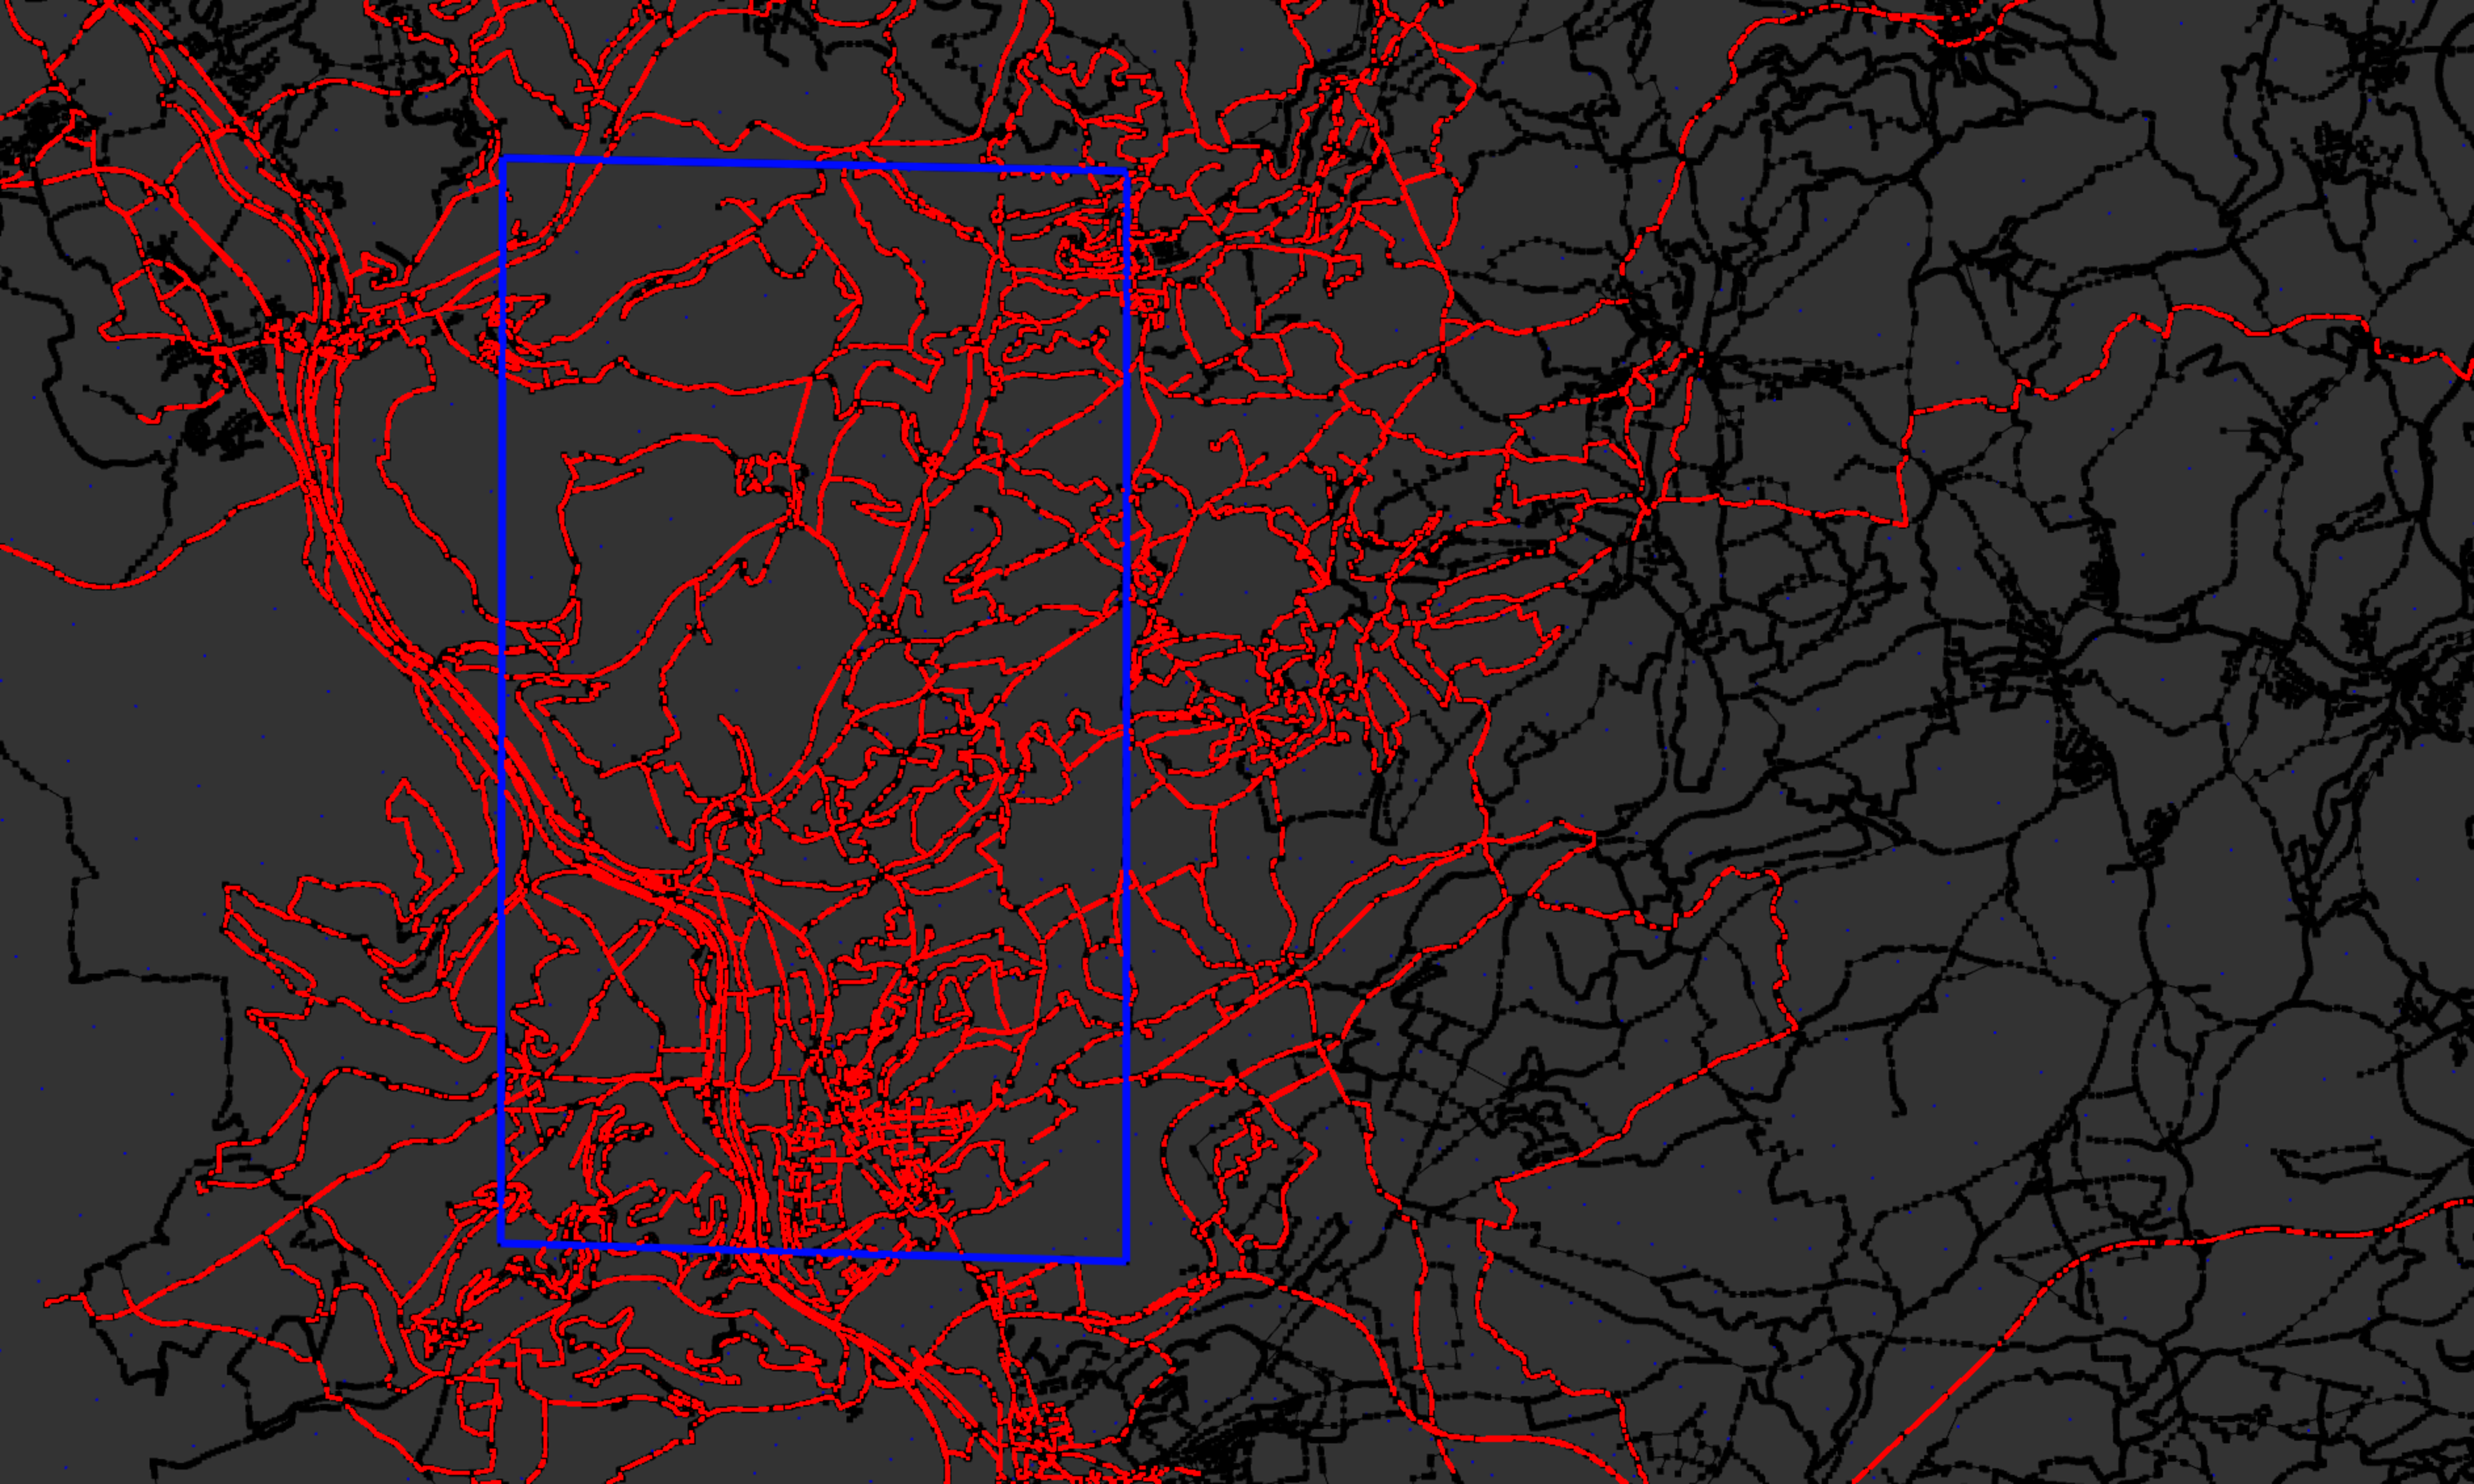
\includegraphics[width=0.75\linewidth]{graphics/saarland_real_data_gimp.pdf}
\end{frame}


\section{Preliminaries}
\begin{frame}
	\frametitle{Contraction Hierarchy}
	\begin{itemize}
		\item Contraction Hierarchy (CH) is an augmentation of a graph $G(V,E,c)$ with \emph{shortcuts} and \emph{node levels}. \pause
		\item \emph{node contraction}: Firstly, remove a node $v$ and all of its adjacent edges from the graph. \pause

		      Then create shortcut $s = (u, w)$ between two adjacent nodes $u,w$ of $v$ if the only shortest path from $u$ to $w$ is the path $uvw$. $c(s) = c(uv) + c(vw)$. \pause
		\item Construct CH by successively contracting all nodes. \pause
		\item final CH data structure is defined as $G(V, E^+, c, l)$ where $E^+$ is the union of $E$ and all shortcuts.
	\end{itemize}
\end{frame}

\begin{frame}
	\frametitle{\chrep}
	\framesubtitle{Compression}
	\begin{figure}
		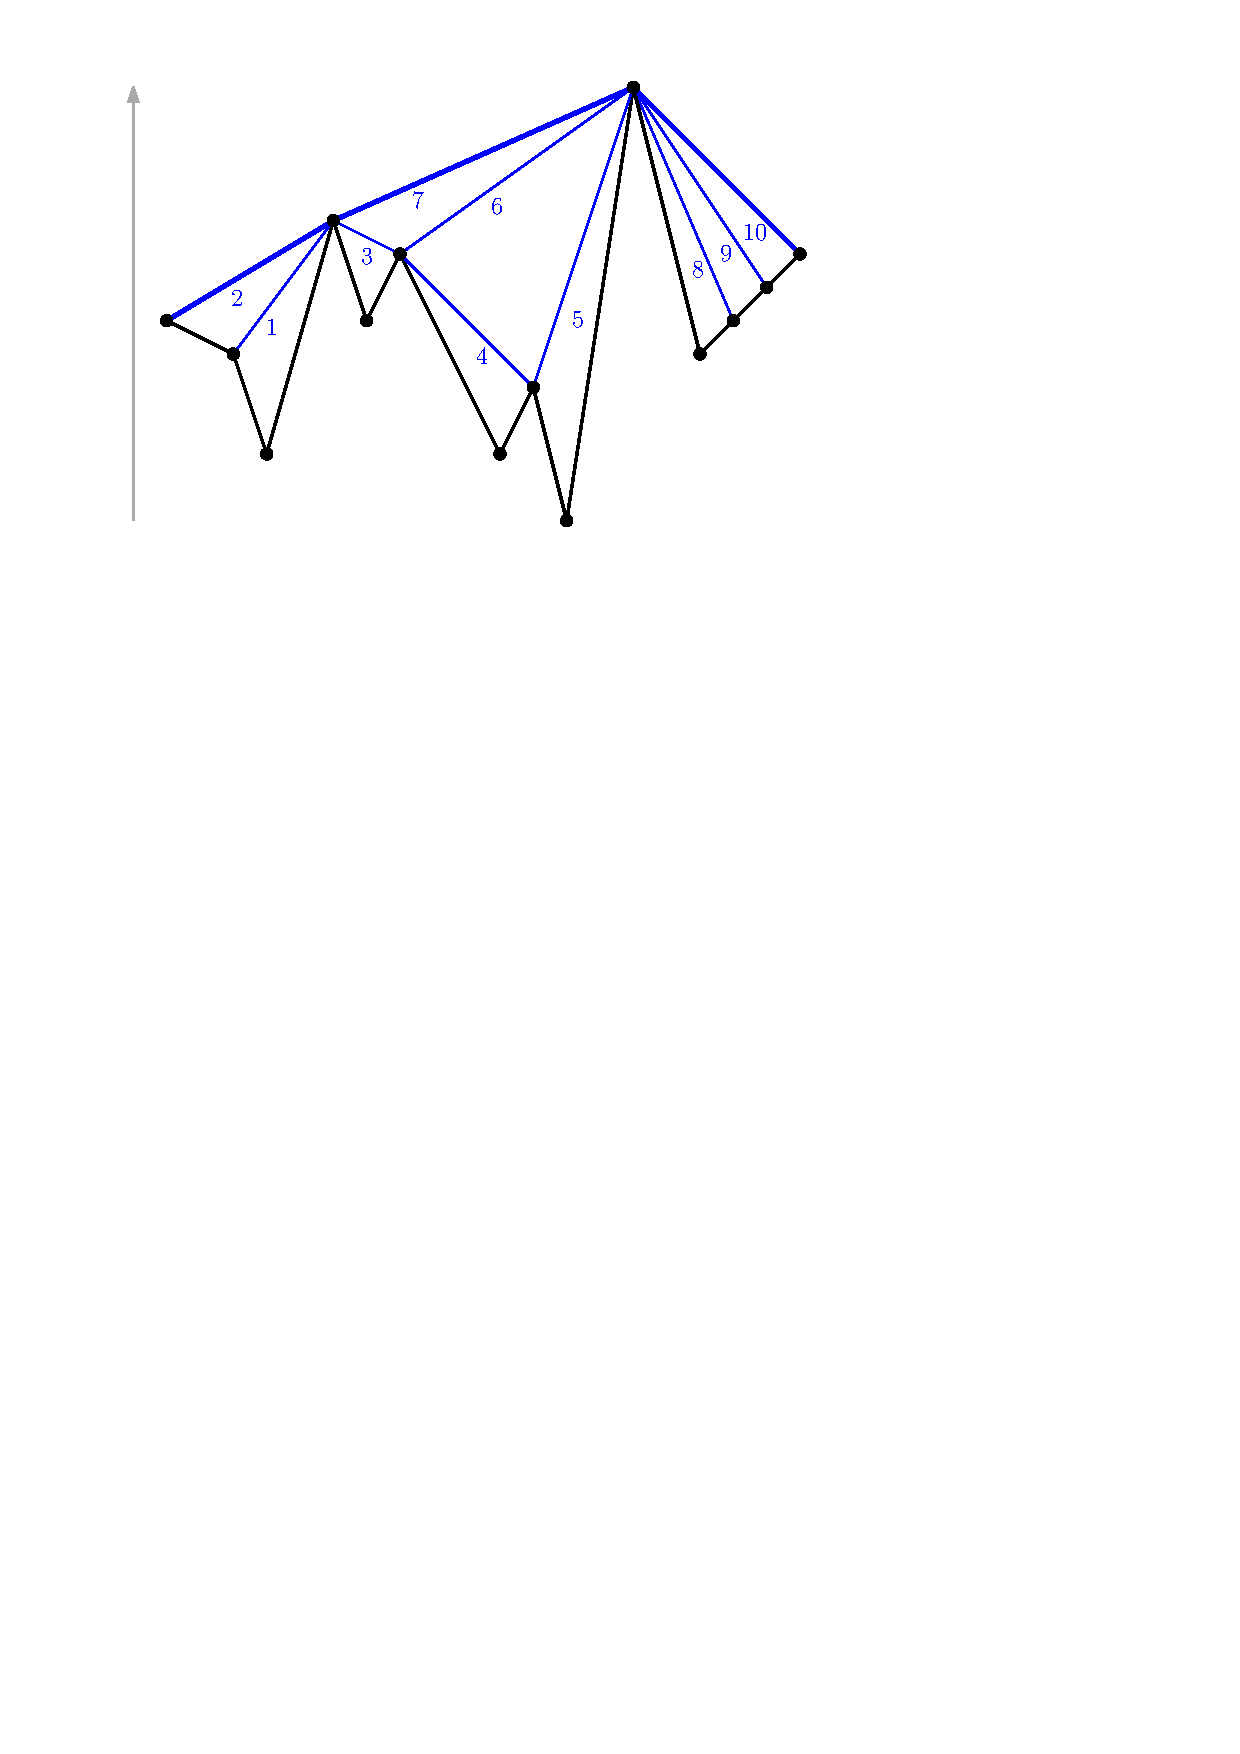
\includegraphics[width=.76\columnwidth]{images/toch}
		\caption{Original path (black) and derivation of its \chrep (bold blue) via repeated shortcut substitution. $y$-coordinate corresponds to CH level.}
	\end{figure}
\end{frame}

\section{Algorithm}

\begin{frame}
	\frametitle{Algorithm Overview}
	Inverted Index: Associate a trajectory with all edges of its \chrep in $E^+$. \pause
	\begin{algorithm}[H]
		\renewcommand{\thealgorithm}{}
		{\small
			\caption{Spatial \pathfinder Algorithm}
			\begin{algorithmic}[1]
				\Procedure{PathfinderQuery}{$Q$} \pause
				\State $E_O \gets \Call{\findEdgeCandidates}{Q}$ \label{line:edge_revrieval} \pause
				\State $E_r \gets \Call{\refineEdgeCandidates}{Q, E_O}$ \pause
				\State \Return $\Call{\getAssociatedTrajectories}{E_r}$
				\EndProcedure
			\end{algorithmic}
			\label{alg:spatial_pathfinder}
		}
	\end{algorithm}
\end{frame}

%\subsection{\findEdgeCandidates}
\begin{frame}
	\frametitle{\findEdgeCandidates}
	\framesubtitle{Path box}
	\emph{Path box} $PB(e)$: Bounding box for the path that an edge $e$ represents:

	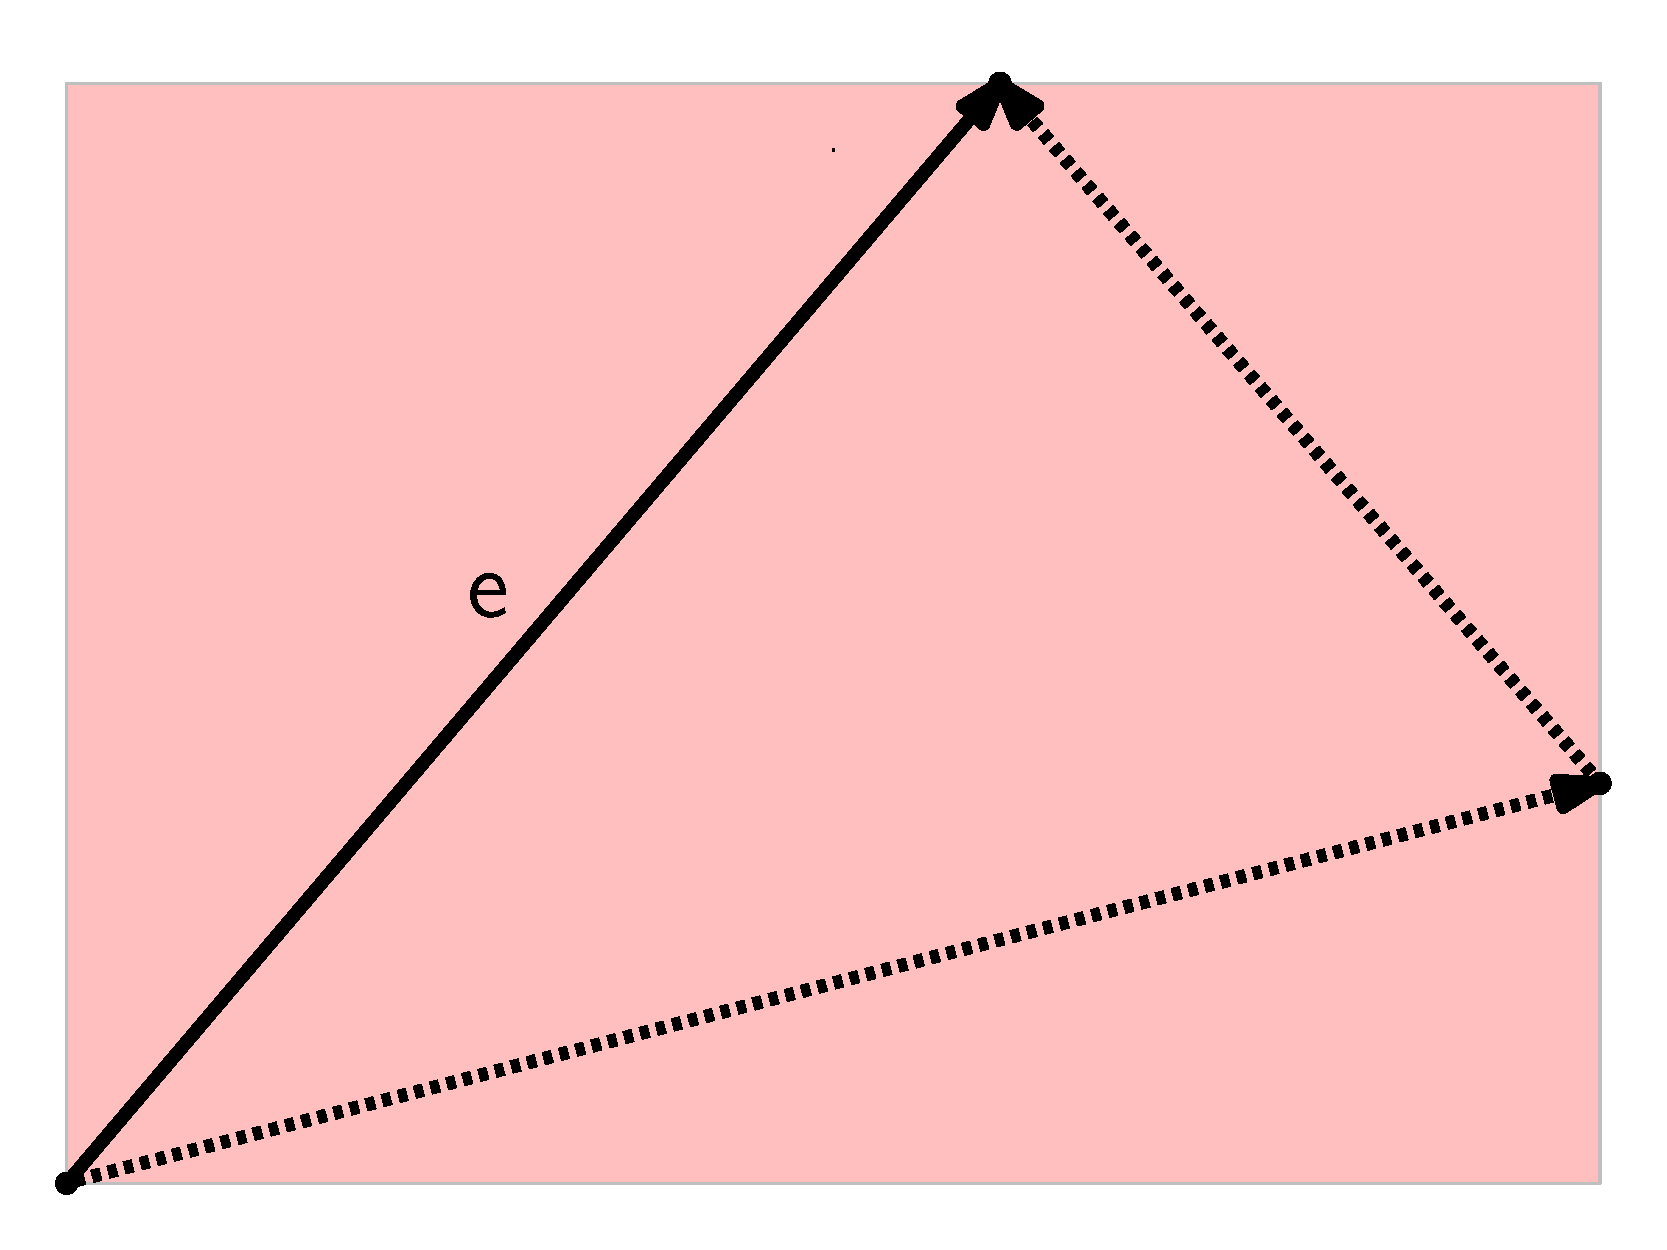
\includegraphics[width=.5\columnwidth]{images/pathBox}
\end{frame}

\begin{frame}
	\frametitle{\findEdgeCandidates}
	\framesubtitle{Downgraph box}
	\emph{Downgraph box} $DB(v)$: Bounding box of all nodes that are reachable from a node $v$ on a down-path (only visiting nodes of decreasing CH-level)
	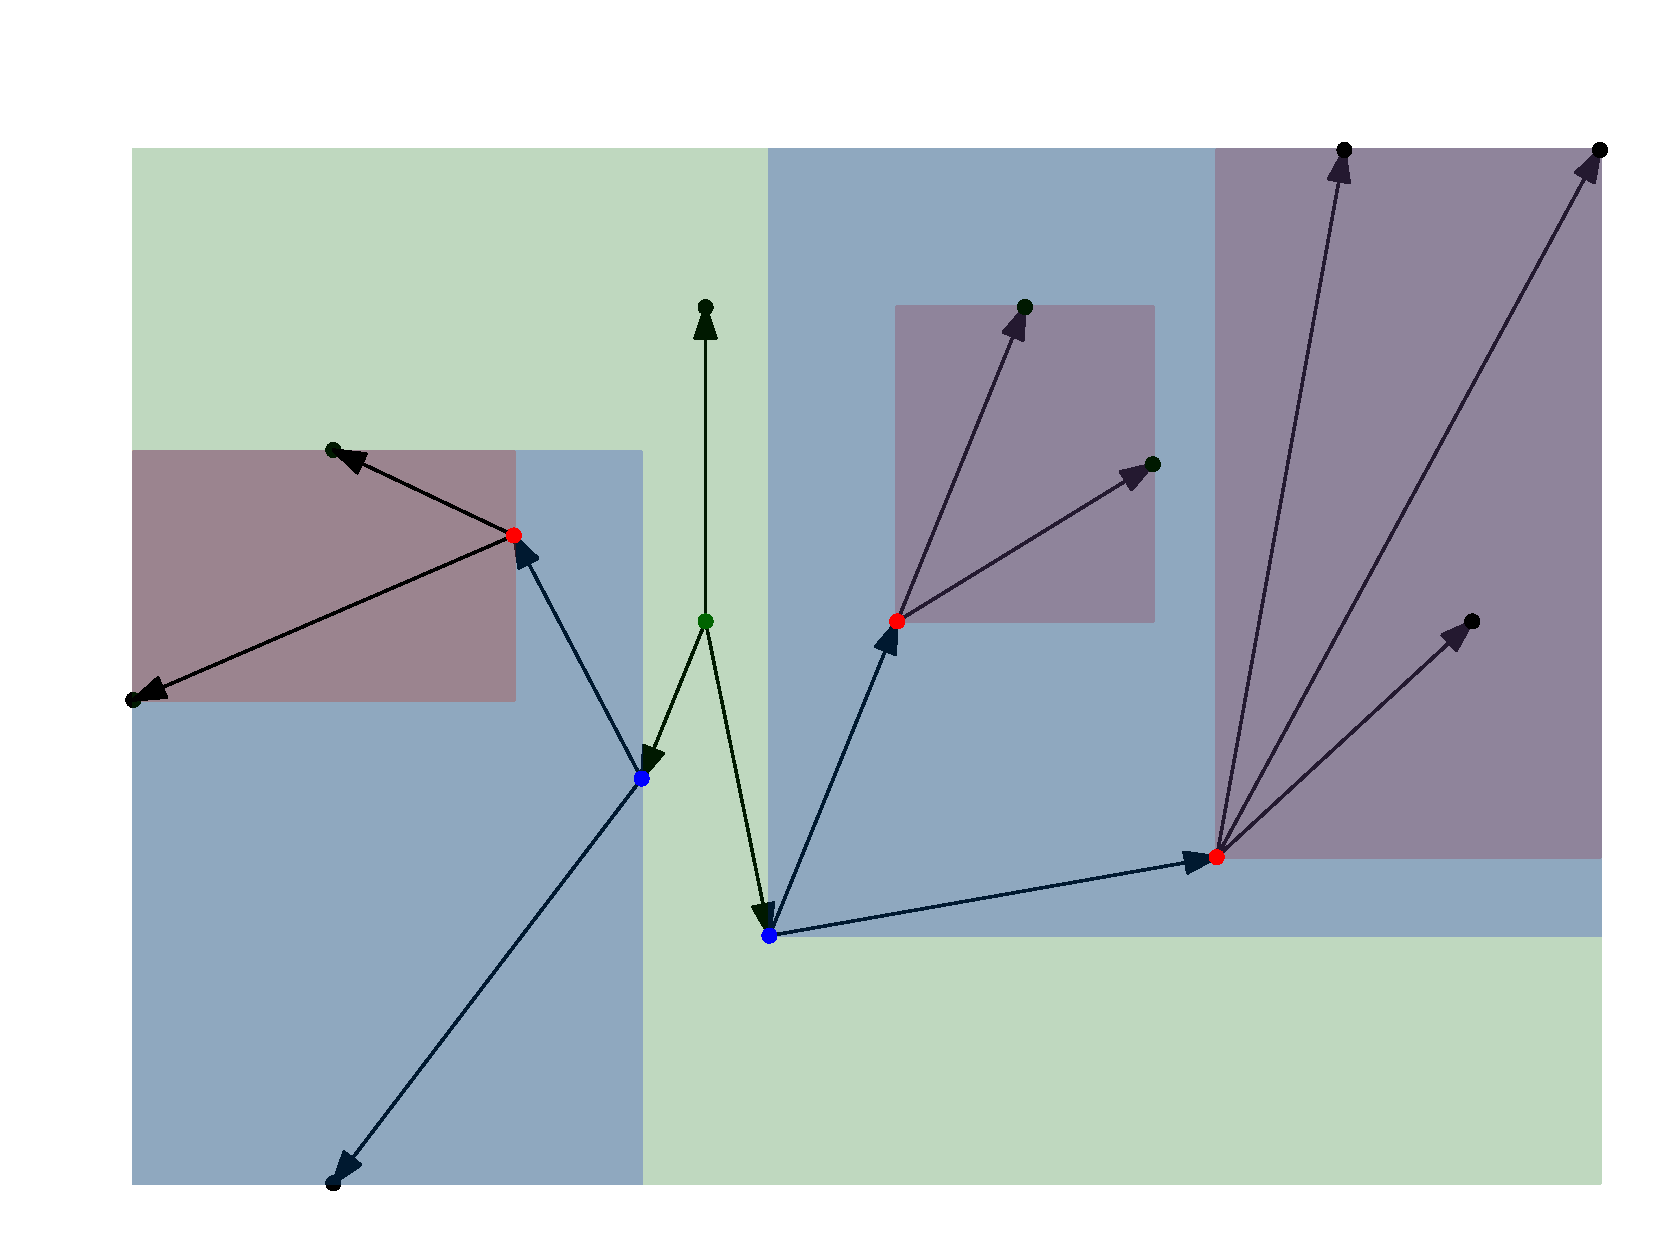
\includegraphics[width=.76\columnwidth]{images/downgraphBox}
\end{frame}

\begin{frame}
	\frametitle{\findEdgeCandidates}
	\begin{algorithm}[H]
		\renewcommand{\thealgorithm}{}
		{\tiny
			\caption{The algorithm to find edge candidates given a query rectangle $Q$.}
			\begin{algorithmic}[1]
				\Procedure{FindCandidatesForNode}{$v, Q$}
				\State $C \gets \emptyset$
				\For {$e \in \text{down edges of $v$}$}
				\If {$PB(e) \cap Q \neq \emptyset$}
				\State $C \gets C \cup \{e\}$
				\EndIf
				\State $v_l \gets \text{lower node of $e$}$
				\If {$DB(v_l) \cap Q \neq \emptyset$}
				\State $C \gets C \cup \Call{FindCandidatesForNode}{v_l, Q}$
				\EndIf
				\EndFor
				\State \Return $C$
				\EndProcedure
			\end{algorithmic}
		}
	\end{algorithm}
	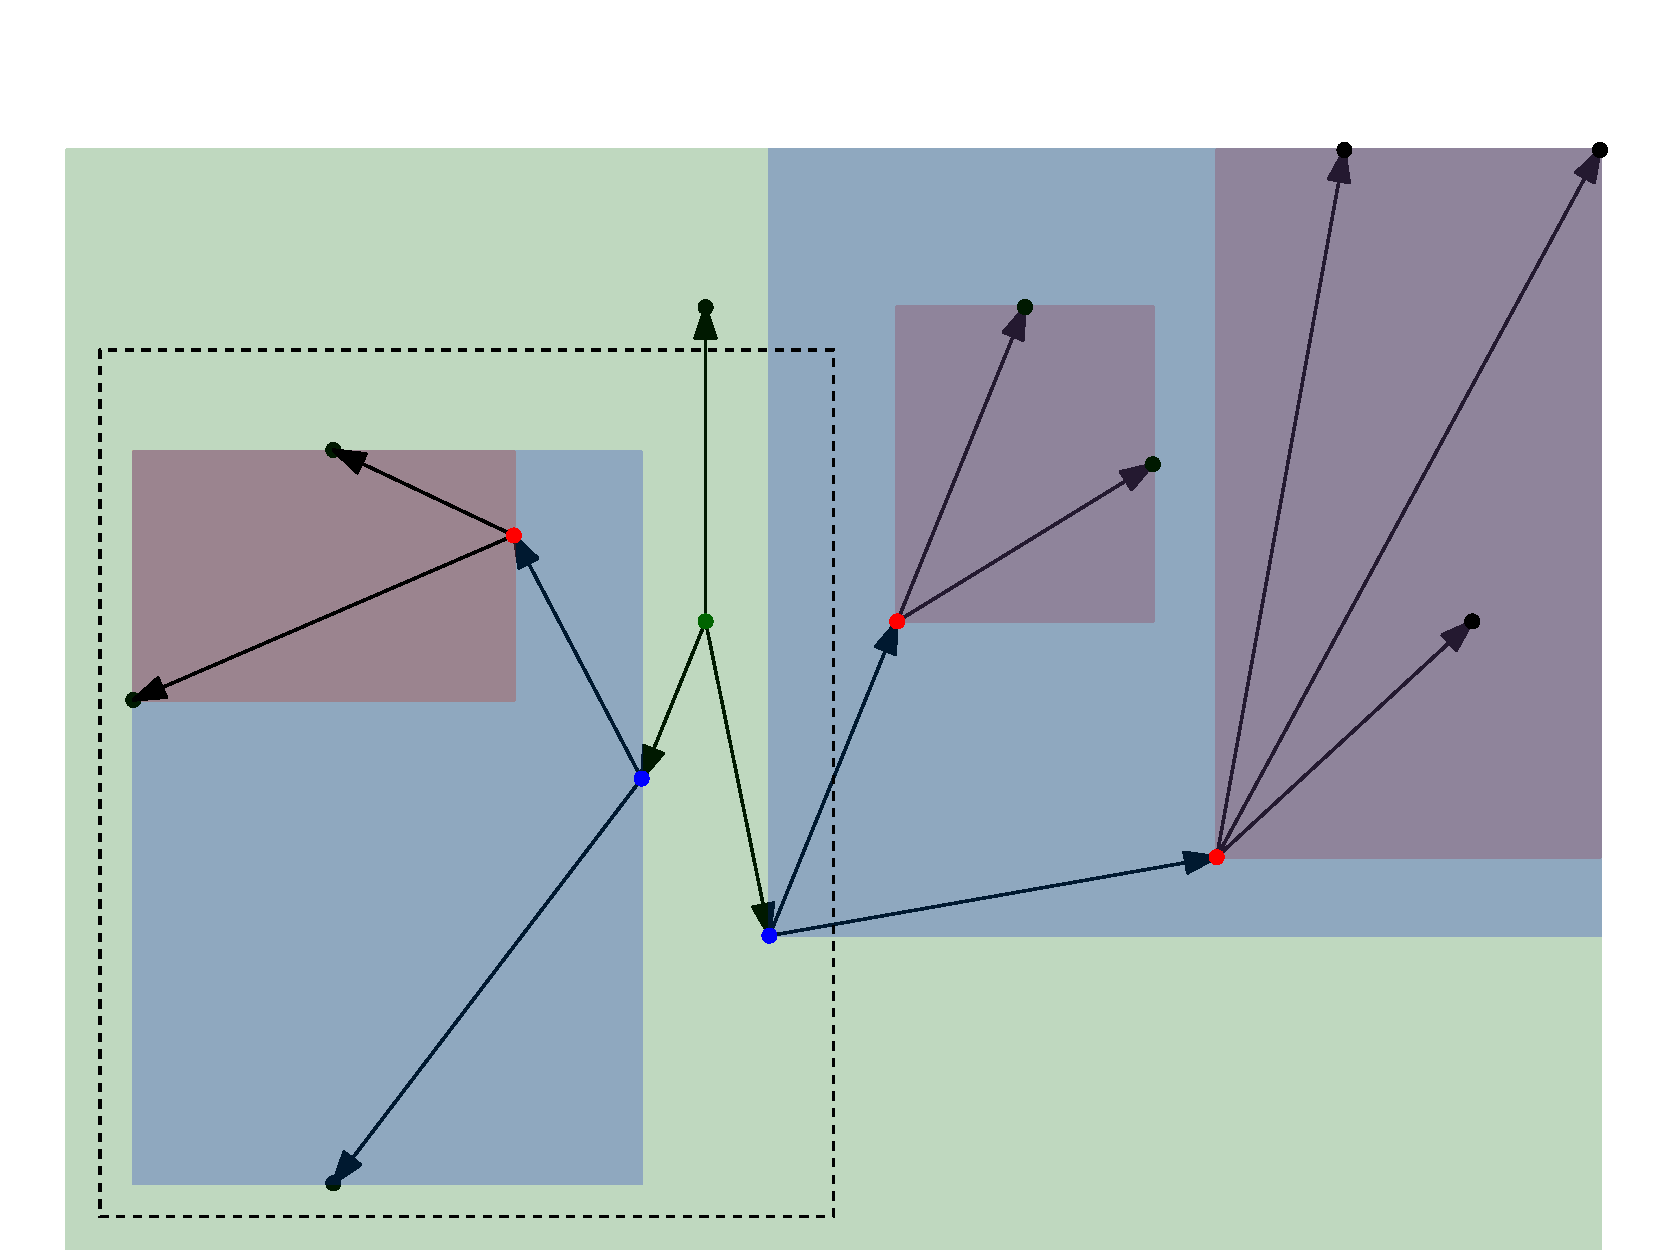
\includegraphics[width=.45\columnwidth]{images/containedDowngraphBox}
\end{frame}

%\subsection{\refineEdgeCandidates}
\begin{frame}
	\frametitle{\refineEdgeCandidates}
	Problem: Some of the candidates my be false positives. \pause

	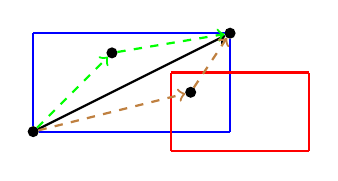
\begin{tikzpicture}

		\SetGraphUnit{1}

		\GraphInit[vstyle=Classic]
		\tikzset{VertexStyle/.style =
				{shape=circle, fill=black, minimum size = 4pt,inner sep=0pt}
		}

		%edge
		\tikzstyle{EdgeStyle}=[->, color=black]
		\SetVertexNoLabel
		\Vertex[x=-0.5,y=2]{source}
		\Vertex[x=2,y=3.25]{target}

		\Edge(source)(target) {e}


		%edgeBox

		\tikzset{VertexStyle/.style =
				{shape=circle, fill=black, minimum size = 0pt,inner sep=0pt}
		}
		\SetVertexNoLabel
		\Vertex[x=2,y=2]{6}
		\Vertex[x=-0.5,y=3.25]{8}

		\tikzstyle{EdgeStyle}=[color=blue]
		\Edge(source)(6)
		\Edge(6)(target)
		\Edge(target)(8)
		\Edge(8)(source)


		%queryBox
		\Vertex[x=1.25,y=1.75]{1}
		\Vertex[x=3,y=1.75]{2}
		\Vertex[x=3,y=2.75]{3}
		\Vertex[x=1.25,y=2.75]{4}

		\tikzstyle{EdgeStyle}=[color=red]
		\Edge(1)(2)
		\Edge(2)(3)
		\Edge(3)(4)
		\Edge(4)(1)

		%unpacked
		\tikzset{VertexStyle/.style =
				{shape=circle, fill=black, minimum size = 4pt,inner sep=0pt}
		}

		%possibility1
		\Vertex[x=0.5,y=3, LabelOut=true, Lpos=-90]{9}

		\tikzstyle{EdgeStyle}=[->, color=green, dashed]
		\Edge(source)(9)
		\Edge(9)(target)

		%possibility2
		\Vertex[x=1.5,y=2.5, LabelOut=true, Lpos=180]{10}

		\tikzstyle{EdgeStyle}=[->, color=brown, dashed]
		\Edge(source)(10)
		\Edge(10)(target)
	\end{tikzpicture}
	\pause

	Here the black edge $e$ is a candidate because of $PB(e) \cap Q \neq \emptyset$. \pause

	If $e$ bridges \pause
	\begin{itemize}
		\item intersecting brown path  $\Rightarrow$ true positive \pause
		\item non-intersecting green path $\Rightarrow$ false positive \pause
	\end{itemize} \pause
	$\Rightarrow$ in doubt, $e$ have to be unpacked recursively
\end{frame}

%\subsection{\getAssociatedTrajectories}
%\begin{frame}
%	\frametitle{\getAssociatedTrajectories}
%	Finally collect all trajectories associated with the remaining candidate edges, i.e. $t \in \bigcup_{e \in E_r} \mathcal{T}_e $.\pause
%
%	Removal of duplicates is also required, as trajectories are associated with more than one edge.
%\end{frame}

\section{Extensions}

%\subsection{Time queries}
\begin{frame}
	\frametitle{Time queries}
	\begin{itemize}

		\item	Two types of time queries: \pause
		      \begin{itemize}
			      \item Time frame queries $[\tau_l, \tau_u]$ \pause
			      \item Time slice queries for periodic events, e.g. Friday Evening \pause
		      \end{itemize}
		\item	Are processed efficiently by interval trees at each edge. \pause

		\item Can be combined with each other and the spatial query. \pause

		\item	Analogues to $PB(e)$ and $DB(v)$ are used, but the compression of time data is lossy.
		      content...
	\end{itemize}
\end{frame}

%\subsection{Parallelization}
\begin{frame}
	\frametitle{Parallelization}
	\begin{itemize}
		\item<1-> Top down CH-traversal in \findEdgeCandidates is a DAG \pause $\Rightarrow$ we can identify a tree such that the traversal can be efficiently parallelized.
		\item<2-> Straightforward to parallelize \refineEdgeCandidates.
		\item<3-> \getAssociatedTrajectories can be parallelized too where the results are finally merged.
	\end{itemize}
\end{frame}

%\subsection{On disk storage}
\begin{frame}
	\frametitle{On disk storage}
	Amount of trajectory data can be too much if RAM is limited \pause

	$\Rightarrow$ Use the library STXXL to store the trajectory data on disk.
\end{frame}

\section{Experiments}

\begin{frame}
	\frametitle{Experiments}
	\framesubtitle{Technology}
	\pathfinder was implemented in C++. \pause
	\medskip

	Experiments were conducted on two machines:
	\begin{enumerate}
		\item AMD Ryzen Threadripper 1950X (16-Core), 128 GB RAM and a 512GB Toshiba OCZ RD400 NVMe SSD (\SI{2.6}{GB}/s)  %3.4 GHz turbo: 4GHz
		\item Intel(R) Xeon(R) CPU E5-2650 v4 (24-Core), 768 GB RAM %turbo 2.9GHz
	\end{enumerate}
\end{frame}

\begin{frame}
	\frametitle{Experiments}
	\framesubtitle{Graph data}
	\begin{table}
		{
			\caption{Characteristics of network graphs, based on Open street Map(OSM)}
			\begin{tabular}{|l|rr|}
				\hline
				                           & Germany  & Europe
				\\ \hline
				\# nodes                   & $57.4M$  & $437.4M$  \\
				\# edges (original)        & $121.7M$ & $902.1M$  \\
				\# edges (CH)              & $248.4M$ & $1694.2M$ \\
				CH construction time (min) & 16       & 125       \\
				\hline
			\end{tabular}
		}
	\end{table}
\end{frame}

\begin{frame}
	\frametitle{Experiments}
	\framesubtitle{Trajectory data}
	Dataset $\traj{ger}{real}$ of 370k real-world trajectories compiled from OSM-traces.
	\begin{table}
		{
			\begin{tabular}{|l|rrr|}
				\hline
				                            & $\varnothing$ & $\sigma$ & max.  \\
				\hline
				\# shortest paths           & 11            & 16.6     & 1118  \\
				length (km)                 & 14.78         & 34.6     & 1928  \\
				original length (\#edges)   & 347           & 654      & 46112 \\
				compressed length (\#edges) & 37            & 56       & 3726  \\
				\hline
			\end{tabular}
		}
	\end{table}
\end{frame}


\begin{frame}
	\frametitle{Experiments}
	\framesubtitle{Index Setup}
	\begin{table}
		{
			\caption{Setting up the auxiliary data structures (CH construction and compression excluded). $|\traj{eu}{synth}| = 10^7$, $d=\SI{e5}{km}$.
			}
			\begin{tabular}{|c|cc|}
				\hline
				           & $\traj{ger}{real}$ & $\traj{eu}{synth}$ \\
				\hline
				setup time & 349s               & 5040s              \\
				total size & 126GB              & 485GB              \\
				\hline
			\end{tabular}
		}

		%init is sum over init() times without partition paths
		%rupp@threadripper:~/osm/benchmarks/germany/papertimes/timeVariants$ vim 16T_results_
		%ruppts@nekton:~/osm/pathfinder/benchmarks/europe/papertimes/timevariants$ vim 10m_24T_results_
	\end{table}
\end{frame}

\begin{table}
	{
		\caption[Messungen$germany\_real\_1_naive_variants_threadripper$]{Timings in seconds for different sized sets $\traj{ger}{synth}$, rectangle size $\frac{1}{32}$, spatial only queries, single thread.
			%Due to the very slow naive approaches this experiment was conducted by averaging only over 10 spatial  queries with rectangle size 1/32 and $d=\SI{100}{km}$ for the generated trajectories.
			% The columns are $|\traj{ger}{synth}|$.
		}
		\begin{tabular}{|l||r|r|r|}
			\hline
			set size          & $100,000$ & $1 M$    & $10 M$
			\\ \hline
			linear scan       & 156.237   & 1568.022 & 15884.508 \\
			inverted index CH & 69.577    & 68.403   & 71.550    \\
			\pathfinder       & 0.029     & 0.107    & 0.415     \\
			\hline
		\end{tabular}
	}
\end{table}

\begin{frame}
	\frametitle{Experiments}
	\framesubtitle{Spatial queries}
	\begin{table}
		\caption[Messungen$europe\_10\_24_spatial_nekton$]{Measurements  for $|\traj{eu}{synth}| = 10^7$ with 24 threads for spatial only queries.}


		\footnotesize
		\centering
		\begin{tabular}{|r||c|c|c|c|c|}
			\hline
			\diagbox[width=40pt]{d}{} & 1/2   & 1/4   & 1/8   & 1/16  & 1/32
			\\\hline
			25km                      & 0.817 & 0.628 & 0.270 & 0.093 & 0.041 \\
			100km                     & 5.630 & 4.381 & 1.866 & 0.609 & 0.201 \\
			400km                     & 6.177 & 4.959 & 2.124 & 0.685 & 0.222 \\
			100000km                  & 6.889 & 4.773 & 1.882 & 0.608 & 0.211 \\
			\hline
		\end{tabular}
	\end{table}
\end{frame}

\begin{frame}
	\frametitle{Experiments}
	\framesubtitle{Time per trajectory}
	\begin{figure}
		\centering
		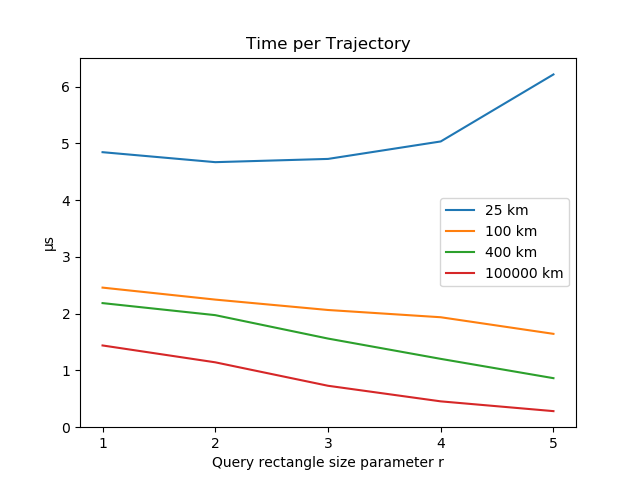
\includegraphics[width=\linewidth]{graphics/time_per_trajectory.png}
		\caption{Time per trajectory in the output for $|\traj{eu}{synth}| = 10^7$ with 24 threads for spatial only query.
			%\STEFAN{So vorgestellt? Das gleiche noch für ger, real? Ist interessanter als ich gedacht habe.  Dass die 25km als einzige wieder hochgeht, hätte ich nicht gedacht.  Das liegt wahrscheinlich daran, dass da so wenige Trajektorien drinliegen und die Schritte b) und c) trotzdem relativ viel kosten.}
		}
	\end{figure}
\end{frame}

\begin{frame}
	\frametitle{Experiments}
	\framesubtitle{Parallelization}
	\begin{figure}
		\centering
		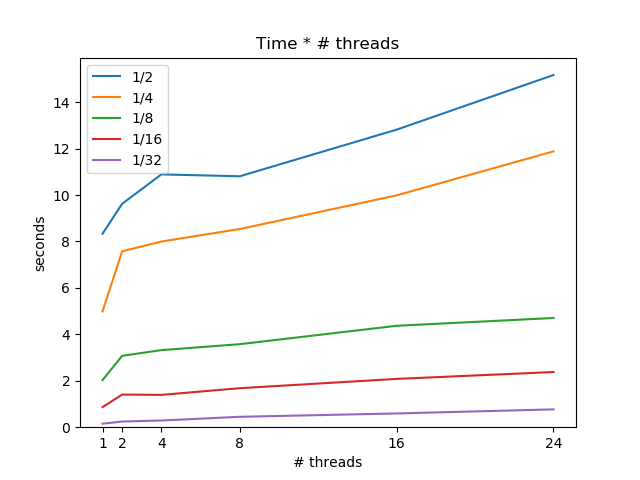
\includegraphics[width=\linewidth]{graphics/normalized_thread_times.png}
		\caption{Table \ref{tab:europe_10m_threadparam_nekton} as a plot with reported times normalized by multiplication with the number of used threads.}
		\label{fig:normalized_thread_times}
	\end{figure}
\end{frame}

\begin{frame}
	\frametitle{Experiments}
	\framesubtitle{Time Queries}
	\begin{table}
		{
			\caption[Messungen$europe\_10\_24_time_variants_nekton$]{Times in seconds for $|\traj{eu}{synth}|=10^7$ with $d=\SI{100}{km}$ and 32 threads for different constraints.}
			\begin{tabular}{|l||c|c|c|c|c|}
				\hline
				                   & 1/2   & 1/4   & 1/8   & 1/16  & 1/32
				\\ \hline
				pure spatial       & 5.630 & 4.381 & 1.866 & 0.609 & 0.201 \\
				intervals          & 1.439 & 1.095 & 0.532 & 0.174 & 0.076 \\
				slices             & 4.273 & 3.412 & 1.449 & 0.461 & 0.157 \\
				intervals + slices & 1.447 & 1.059 & 0.520 & 0.168 & 0.068 \\
				\hline
			\end{tabular}
		}
	\end{table}
\end{frame}

\begin{frame}
	\frametitle{Experiments}
	\framesubtitle{Quality loss due to temporal resolution}
	\begin{table}
		{
		\caption{Size of result set $\mathcal{T}_{\text{out}}$: quality loss due to decrease of temporal resolution (averaged over 2000 queries).}\label{tab:temporalQualityLoss}
		\begin{tabular}{|l||r|r|r|r|r|}
			\hline
			                                                & 1/2      & 1/4      & 1/8     & 1/16    & 1/32   \\
			\hline
			uncompressed                                    & 959.8600 & 313.8005 & 98.2340 & 28.5760 & 9.6105 \\
			compressed                                      & 960.3985 & 314.2435 & 98.4980 & 28.7365 & 9.6890 \\
			$\frac{\text{uncompressed}}{\text{compressed}}$ & 0.999    & 0.998    & 0.997   & 0.994   & 0.991  \\
			\hline
		\end{tabular}
		}
	\end{table}
\end{frame}

\begin{frame}
	\frametitle{Experiments}
	\framesubtitle{On Disk Storage}
	\begin{table}
		{
			\caption{On disk and RAM results for step \getAssociatedTrajectories and $|\mathcal{T}_{out}|$, single thread.}
			\begin{tabular}{|l||r|r|r|r|r|}
				\hline
				                          & 1/2   & 1/4   & 1/8  & 1/16 & 1/32 \\
				\hline
				On disk (\SI{}{s})        & 36.33 & 22.60 & 9.35 & 3.86 & 1.53 \\
				RAM (\SI{}{s})            & 19.20 & 10.67 & 3.56 & 1.11 & 0.26 \\
				$|\mathcal{T}_{out}|$ (M) & 16.49 & 12.46 & 6.80 & 3.46 & 1.42 \\
				\hline
			\end{tabular}
		}
	\end{table}
\end{frame}

\begin{frame}
	\frametitle{Experiments}
	\framesubtitle{Edge-trajectory association}
	\begin{figure}
		{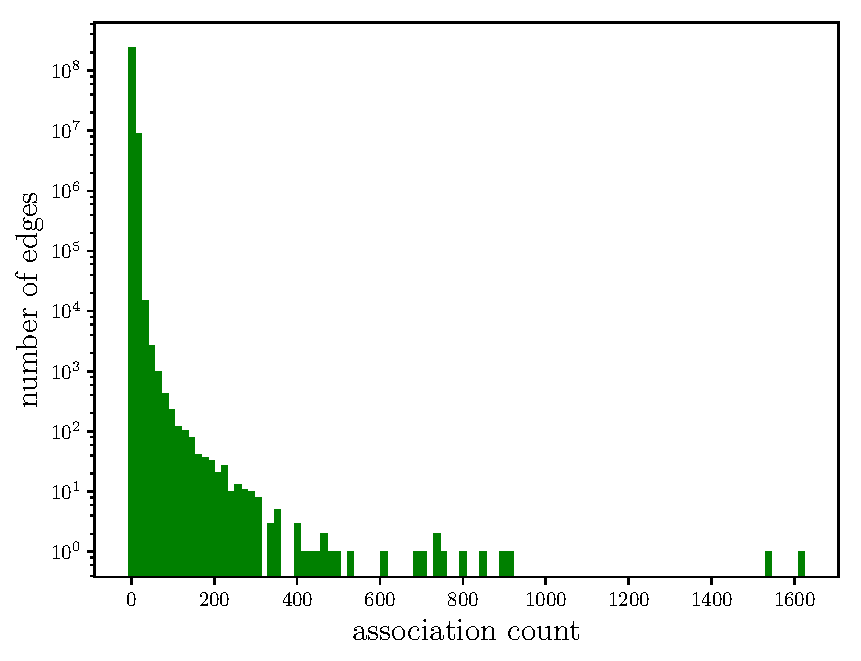
\includegraphics[width=.4\linewidth]{plots/osmGerHist.pdf} }
		\caption{Edge-trajectory associations histogram  for $\traj{ger}{real}$.}
	\end{figure}
\end{frame}

% etc
\end{document}
